\documentclass[10pt,a4paper,twocolumn]{article}
\usepackage[utf8]{inputenc}
\usepackage[T1]{fontenc}
\usepackage[margin=1.55cm,top=1.75cm,bottom=1.75cm,columnsep=0.6cm]{geometry}
\usepackage{graphicx}
\usepackage{booktabs}
\usepackage{amsmath,amssymb}
\usepackage{array}
\usepackage{caption}
\usepackage{xcolor}
\usepackage{hyperref}
\usepackage{float}

\captionsetup{font=small,labelfont=bf,skip=4pt}
\definecolor{darkblue}{RGB}{20,50,110}
\hypersetup{
    colorlinks=true,
    linkcolor=darkblue,
    citecolor=darkblue,
    urlcolor=darkblue
}

\setlength{\parskip}{3.5pt}
\setlength{\parindent}{1em}

\title{\vspace{-0.8cm}\textbf{\Large Macroevolution, Assembly Audits, Telomeric Divergence, and Pleiotropic Rate Constraints Shaping Lifespan, Brain Size, and Cancer Vulnerability in Parrots}}

\author{
\textbf{Angelo}\\
\small Centro Universit\'ario do Planalto Central Apparecido dos Santos (UNICEPLAC), Bras\'ilia, DF, Brazil\\
\small Reproducible repository: \texttt{github.com/redkk123/Parrots} (\texttt{claude/new-session-lwh7xh})
}

\date{\small November 10, 2026 --- Complete Pre-Registered Study, 71-Species Extension, 3D Structural Mapping \& 9-Point Red-Team Statistical Audit}

\begin{document}

\twocolumn[{
  \begin{@twocolumnfalse}
    \maketitle
    \vspace{-0.4cm}
    \begin{abstract}
    \noindent \textbf{Abstract.} Parrots (order Psittaciformes) combine extreme longevity (30 to $>60$ years in macaws, cockatoos, Amazons, and \textit{Strigops habroptila}) and primate-like encephalization with short-lived, neoplasia-prone lineages such as the budgerigar (\textit{Melopsittacus undulatus}). Under a pre-registered three-phase protocol, we combined comparative neoplasia epidemiology ($15,881$ necropsies across AZA and UC Davis databases), phylogenetic comparative allometry and Ornstein-Uhlenbeck regime-shift modeling across two topologies (Burgio et al.\ 2019 supertree, $n = 413$; Smith et al.\ 2024 molecular phylogeny, $n = 399$), comprehensive quality and taxonomic verification of $126$ genome assemblies (\texttt{compleasm aves\_odb10}, Mash nuclear divergence, and mitogenome BLAST), branch-site and selection-intensity tests across a 101-gene panel (modules M1--M8, $58$-species discovery + $71$-species confirmatory extension, benchmarked against $298$ control genes and raw SRA reads), AlphaFold 3D domain mapping, and genome-wide relative evolutionary rate scans (\texttt{RERconverge}, $7,756$ genes, $1,000$ Brownian permulations) subjected to a nine-point adversarial ``Red-Team'' audit. Macroevolutionary analyses support a long-lived ancestral regime (root optimum $+0.22$) followed by a topology-sensitive lifespan reduction in Psittaculidae ($p = 0.003$ Burgio vs.\ $p = 0.050$--$0.052$ Smith, $\lambda = 0.88$), while veterinary necropsies pinpoint extreme tumor incidence uniquely to \textit{M.\ undulatus} ($20.8\%$ AZA / $25.9\%$ age-standardized UC Davis vs.\ $1.5$--$5.4\%$ in lories, OR $= 17, p \le 10^{-16}$). Auditing $126$ assemblies uncovered cross-species mitogenome contamination in $61/96$ Iridian short-read genomes and four severe nuclear swaps/chimeras, yielding $71$ validated species ($\text{BUSCO} \ge 70\%$, zero technical bias with longevity, $p \ge 0.11$). Across tumor-suppressor modules (H8), we refute gene loss or relaxed selection: all $329$ initial disrupted calls in $58$ species ($451$ in $71$ species) proved to be reference-divergence, heterozygous, or high-GC exon-1 coverage dropouts, and no module deviated from the $298$-gene null after correction. Standard \texttt{aBSREL} flagged episodic divergence in $5/8$ ($62.5\%$) telomeric M7 genes (\texttt{RTEL1}, \texttt{TERF2}, \texttt{TERT}, \texttt{ACD}, \texttt{TERF1}) plus \texttt{MYC} on \textit{M.\ undulatus} (vs.\ $0/19$ FDR in control genes, Fisher $p = 0.00069$), confirmed as 100\% orthologous via \textit{S.\ habroptila} dual-reference coordinates; however, window cleaning removes \texttt{RTEL1}, \texttt{ACD}, and \texttt{TERF2}, and \texttt{Double+Triple} multinucleotide models absorb all five ($p = 0.967$--$1.00$), implicating clustered C-terminal (\texttt{RTEL1}) and OB-domain (\texttt{POT1}) multinucleotide dynamics rather than dispersed positive selection. Genome-wide (H6), unadjusted longevity- and brain-associated \texttt{RER} profiles correlate at $r = 0.666$--$0.667$, yet our Red-Team audit reveals that true OLS/branch orthogonalization halves residual brain coupling ($r = 0.332$--$0.389$ vs.\ $0.639$ from unwhitened PGLS residuals), phenotypic covariance depends heavily on Psittaculidae ($r_{\text{tip}}$ drops from $0.478$ to $0.195$), and $89.3\%$ ($117/131$) of shared candidate hits (\texttt{PTEN}, \texttt{MAD2L2}, \texttt{HSPA8}, \texttt{CTNNB1}) have $97$--$99\%$ zero-length branches mirroring the genomic background vector $\pm\sqrt{\text{nv}}$. Partitioning hits into Tier~A (ultra-conserved background-coupled) and Tier~B ($14$ informative genes with $\ge 20$ nonzero branches, led by \texttt{TKT}, \texttt{PHOSPHO1}, \texttt{SLC4A7}, and \texttt{HUS1}) establishes a rigorous benchmark for avian comparative genomics.\par\vspace{4pt}
    \noindent\textbf{Keywords:} Psittaciformes $\cdot$ Peto's Paradox $\cdot$ Longevity $\cdot$ Encephalization $\cdot$ Telomeres (\texttt{RTEL1}, \texttt{TERT}) $\cdot$ \texttt{PTEN} $\cdot$ \texttt{RERconverge} $\cdot$ Statistical Audit
    \end{abstract}
    \vspace{0.2cm}
  \end{@twocolumnfalse}
}]

\section{Introduction}

Understanding how large, long-lived, and highly encephalized vertebrates suppress somatic malignancy over multi-decade lifespans remains a foundational question at the intersection of evolutionary biology, oncology, and neuroscience (Peto's paradox). Among endothermic vertebrates, parrots (order Psittaciformes) occupy an exceptional evolutionary space. Despite elevated avian metabolic rates and high plasma glucose, macaws (\textit{Ara}, \textit{Anodorhynchus}), cockatoos (\textit{Cacatua}, \textit{Probosciger}), Amazons (\textit{Amazona}), and the flightless kakapo (\textit{Strigops habroptila}) regularly survive 30 to over 60 years while evolving telencephalic neuron counts comparable to primates. Conversely, within the Old World family Psittaculidae, small species such as the budgerigar (\textit{Melopsittacus undulatus}) exhibit brief lifespans and extraordinarily high frequencies of spontaneous neoplasia in veterinary pathology series.

Prior genomic studies of parrot longevity and cognition relied primarily on pairwise comparisons of a few long-lived taxa against non-parrot outgroups (e.g., Wirthlin et al.\ 2018). Yet order-wide comparative genomics has recently been reshaped by hundreds of low-cost short-read draft assemblies deposited into public repositories (such as the Iridian Genomes project; Hains et al.\ 2022), alongside two competing phylogenies (Burgio et al.\ 2019 supertree vs.\ Smith et al.\ 2024 sequence-based phylogeny). Without systematic assembly auditing, short-read fragmentation, cross-sample contamination, and high-GC exon dropout can manufacture false signals of gene loss or accelerated molecular evolution, while uncalibrated macroevolutionary rate correlations can mistake shared clade structure or genome-background normalization artifacts for independent gene-level convergence.

Here we report the complete execution of a pre-registered three-phase investigation (\texttt{results/phase0/analysis\_plan.md}), augmented with AlphaFold 3D structural mapping, a 71-species confirmatory panel extension, and an exhaustive nine-point Red-Team statistical audit designed explicitly to falsify our own primary claims.

\section{Materials and Methods}

\subsection{Phase 0 \& 0b: Phylogenies, Traits, Regime Shifts, and Necropsy Epidemiology}
Life-history data were curated from Smeele et al.\ (2022; BaSTA Gompertz captive life expectancy at birth, $n = 218$ species with matched adult body mass in the 413-tip Burgio et al.\ 2019 supertree), sample-size-adjusted maximum longevity records from AnAge and the Amniote Life History Database ($n = 152$ adjusted, $171$ unadjusted), and endocranial/brain mass ($n = 186$). Models were cross-checked against the phylogenomic tree of Smith et al.\ (2024; $399$ sequence-backed species). Phylogenetic generalized least squares (PGLS, Pagel's $\lambda$ implemented in Python and validated to $<10^{-4}$ against \texttt{nlme::gls} and \texttt{phylolm} in R) quantified allometric slopes and trait residuals. Evolutionary regime shifts across the supertree were inferred with scalar Ornstein-Uhlenbeck expectation-maximization (\texttt{PhylogeneticEM}, $K = 0$--$12$, LINselect criterion). Statistical power was simulated under bivariate Brownian motion across the $n = 105$ genome-matched species set.

To determine whether elevated cancer vulnerability characterizes Psittaculidae broadly or \textit{M.\ undulatus} specifically, we analyzed two independent veterinary pathology registries: (1) AZA zoological necropsies (Kapsetaki et al.\ 2024; $5,729$ necropsies across $108$ bird species including $15$ parrots) tested with beta-binomial models and Fisher's exact tests, and (2) the UC Davis / Drury R.\ Reavill clinical pathology database ($10,152$ parrot necropsies with $\ge 3$ examined tissues), applying direct age standardization to rule out captive age-structure confounding.

\subsection{Phase 1: Systematic Audit of 126 Genome Assemblies}
All 126 NCBI assemblies matching species with trait data ($96$ Iridian short-read Illumina/SPAdes drafts + $30$ chromosome-scale or long-read genomes from VGP, B10K, Wellcome Sanger, and BGI) were downloaded on-the-fly, evaluated, and removed to minimize storage footprint. Gene completeness was measured via \texttt{compleasm} v0.2.10 against \texttt{aves\_odb10} ($8,338$ orthologs). To detect sample swaps and library cross-contamination, mitogenome contigs identified via \textit{COX1}/\textit{CYTB}/\textit{ND2} from five divergent parrots were queried against $6,700$ GenBank avian vouchers strictly \textit{excluding} Iridian/Hains/Pirro records. Nuclear distances across $176$ assemblies ($96$ Iridian + $48$ independent replicates + $32$ putative donor species) were computed using Mash v2.3 ($k = 21$, $50,000$ hashes). Pre-registered inclusion rules required $\text{BUSCO}_{\text{complete}} \ge 70\%$, passing nuclear Mash placement ($\text{residual} \le 0.006$ at $\text{N50} \ge 5\text{ kb}$), and deduplication to one best assembly per species, yielding $71$ validated species ($58$ frozen discovery on Oct.\ 28, 2026 + $13$ newly finalized holdouts). Quality bias was tested via PGLS of residual longevity against BUSCO completeness, $\log_{10}(\text{contig N50})$, GC\%, and assembly length deviation.

\subsection{Phase 2: Proteome Extraction, H8 Panel, Null Pool, SRA Validation, and 71-Species Extension}
All $16,045$ canonical \textit{M.\ undulatus} RefSeq proteins were aligned against every approved genome via \texttt{miniprot} v0.18 (\texttt{-outn=3}, scoring ORFs as \textit{complete} when coverage $\ge 90\%$, identity $\ge 60\%$, and free of frameshifts or premature stops). In the $58$-species discovery panel ($15$ Psittaculidae, $43$ non-Psittaculidae), codon alignments (\texttt{MAFFT} + \texttt{PAL2NAL}) were constructed for $101$ candidate genes partitioned across eight pre-specified modules: M1 (p53/cell cycle), M2 (PI3K/mTOR/proliferation), M3 (apoptosis), M4 (DNA DSB/BER repair), M5 (NRF2/xenobiotics), M6 (antioxidants), M7 (telomere/shelterin), and M8 (proteostasis/autophagy). We evaluated relaxation/intensification in Psittaculidae (stem + internal branches as \texttt{TEST}) with \texttt{HyPhy RELAX} (\texttt{-{}-models Minimal}) and episodic positive selection on the Psittaculidae stem and \textit{M.\ undulatus} tip branch with \texttt{HyPhy aBSREL} across both topologies. Benjamini-Hochberg FDR was applied across all testable panel genes per tree ($86$--$87$ genes) on top of HyPhy's per-gene Holm-Bonferroni correction across the two test branches. Modular statistics (proportion relaxed at $q < 0.10, k < 1$ and mean $\log_2 k$) were benchmarked against $10,000$ module-label permutations and $1,000$ length- and background-rate-matched pseudo-panels sampled from $298$ genomic control genes. Disrupted calls were verified against a second long-lived reference proteome (\textit{Strigops habroptila}) and raw Illumina SRA reads (\texttt{bwa-mem2}/\texttt{samtools}). Upon finishing Phase 1, all $97$ alignable H8 panel genes were also extended to the full $71$-species cohort (\texttt{results/phase2\_genes\_71sp/}) with confirmatory \texttt{RELAX} and \texttt{aBSREL} verification on key H8 genes.

\subsection{Phase 3: Genome-Wide \texttt{RERconverge}, 3D Mapping, and 9-Point Red-Team Audit}
Across $7,756$ coding genes with intact ORFs in $\ge 50\%$ of the $58$ discovery species, amino-acid branch lengths were optimized under LG (\texttt{phangorn::optim.pml}) on both topologies. Relative evolutionary rates (\texttt{RERconverge} v0.3.0, \texttt{getAllResiduals}, square-root transform, weighted, column-scaled) were correlated (\texttt{winsorize = 3}) with \texttt{rel\_log\_life\_expectancy} ($n = 58$), \texttt{rel\_log\_brain} ($n = 50$), and \texttt{rel\_brain\_given\_le} ($n = 50$), plus within-Psittaculidae ($n = 15$) and within-rest ($n = 43$) subsets, using $1,000$ topology-conditioned Brownian motion permulations (\texttt{Rcpp fastCorPerms}). Enrichment was tested over $1,780$ GO Biological Process terms ($\ge 10$ genes, \texttt{fastWilcoxGMTAll}) and six pre-declared exploratory functional axes. AlphaFold structures for \texttt{POT1}, \texttt{RTEL1}, \texttt{PTEN}, and \texttt{MAD2L2} were segmented by Predicted Aligned Error (PAE) to map lineage-specific substitutions.

Finally, nine adversarial Red-Team audits tested: (1) seed reproducibility (`seed=20261028` vs `999999`), (2) negative control traits and $200$-replicate Brownian null distributions for genome-wide coupling $r$, (3) technical confounders (length, tree length, GC3, missingness, gaps) and zero-branch invariance, (4) leave-one-clade-out perturbations, (5) true tip-OLS, branch-path, and analytical partial orthogonalization of \texttt{rel\_brain\_given\_le}, (6) empirical \texttt{aBSREL} base rates across control genes, (7) \texttt{MAFFT L-INS-i}, stringent gap/cluster window masking, \texttt{Double+Triple} multi-hit models, and kakapo dual-reference coordinate concordance in telomeric genes, (8) 71-species panel / 13-species holdout and 30-split cross-validation replication, and (9) an exhaustive statistical inventory of all $78,802$ tests and null outcomes.

\begin{figure*}[t]
\centering
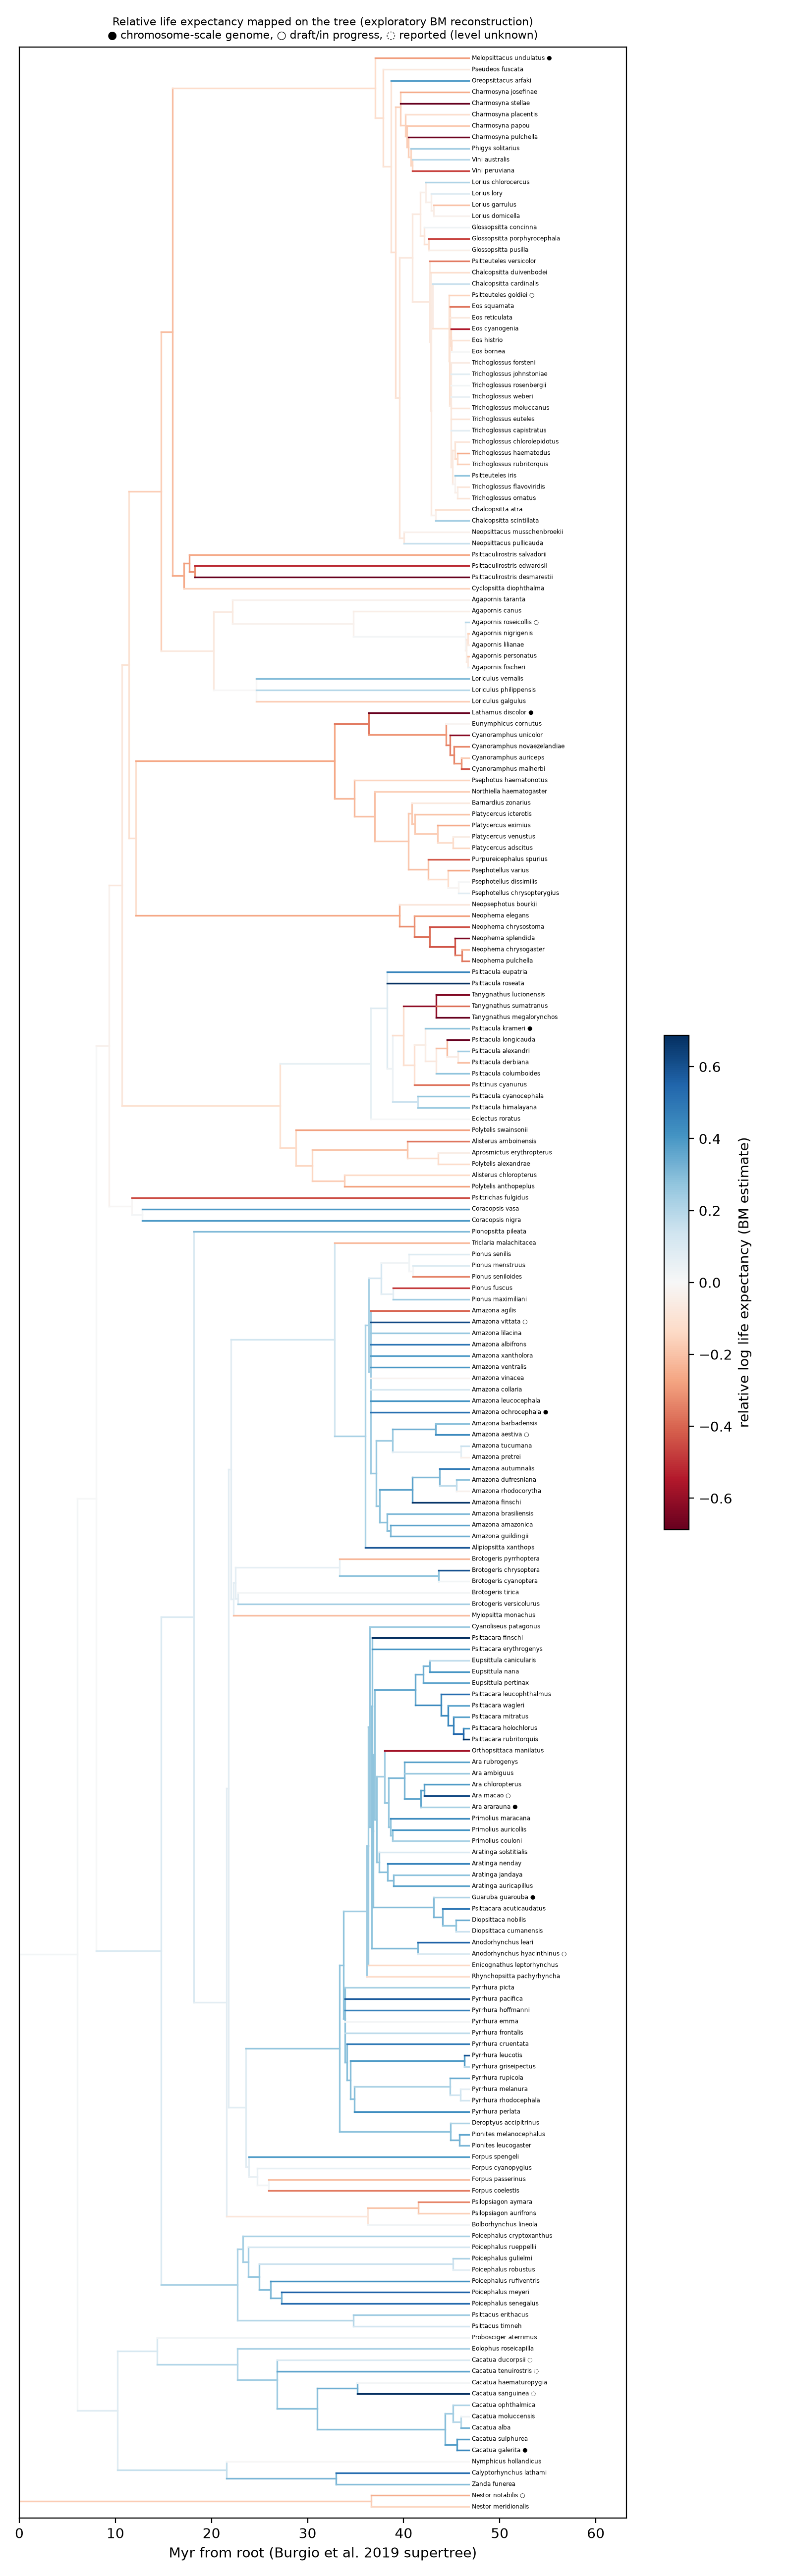
\includegraphics[width=0.48\textwidth]{../results/phase0/figures/fig1_tree_relative_LE.png}\hfill
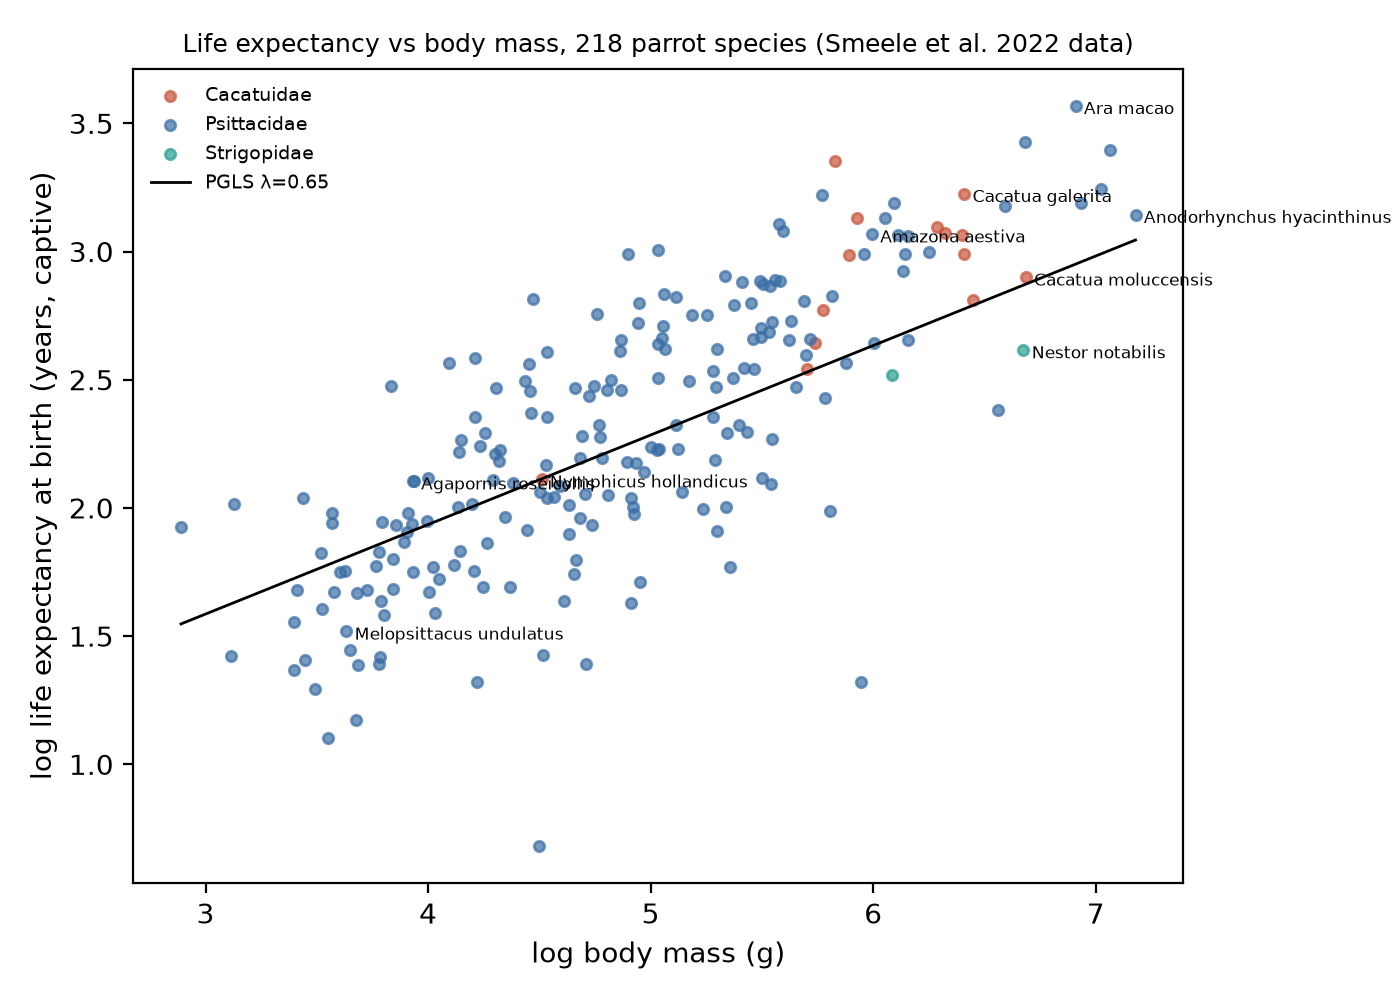
\includegraphics[width=0.48\textwidth]{../results/phase0/figures/fig2_allometry.png}
\caption{\textbf{Phase 0 Macroevolutionary Baseline ($n = 218$ species):} (\textbf{Left}) Ancestral reconstruction of relative captive life expectancy across the Burgio 2019 Psittaciformes supertree. (\textbf{Right}) Allometric scaling of life expectancy ($\beta_{\text{PGLS}} = 0.349 \pm 0.032$, $\lambda = 0.65$) and brain mass across parrots relative to non-psittaciform birds.}
\label{fig:phase0}
\end{figure*}

\begin{figure*}[t]
\centering
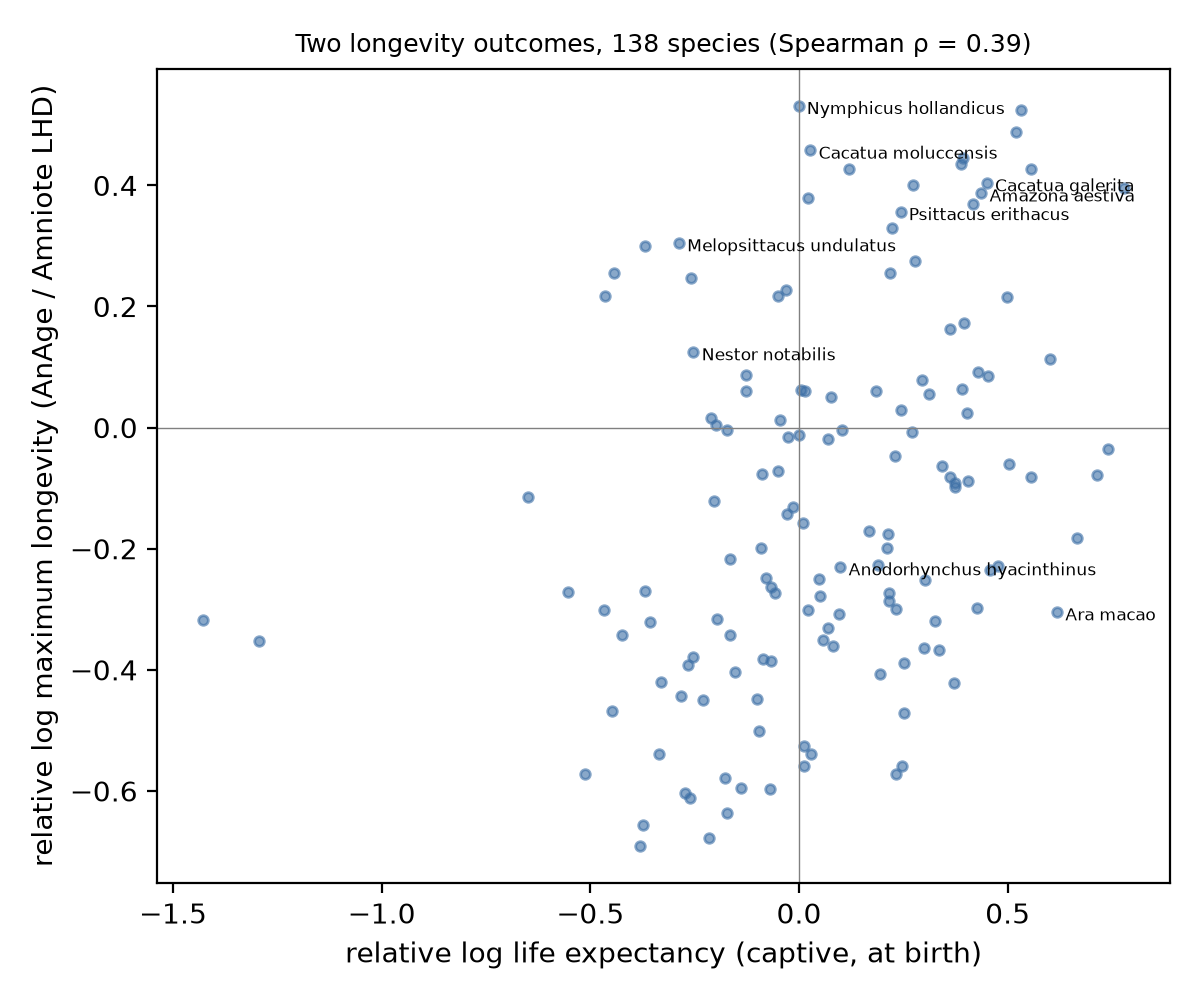
\includegraphics[width=0.48\textwidth]{../results/phase0b/figures/fig3_two_outcomes.png}\hfill
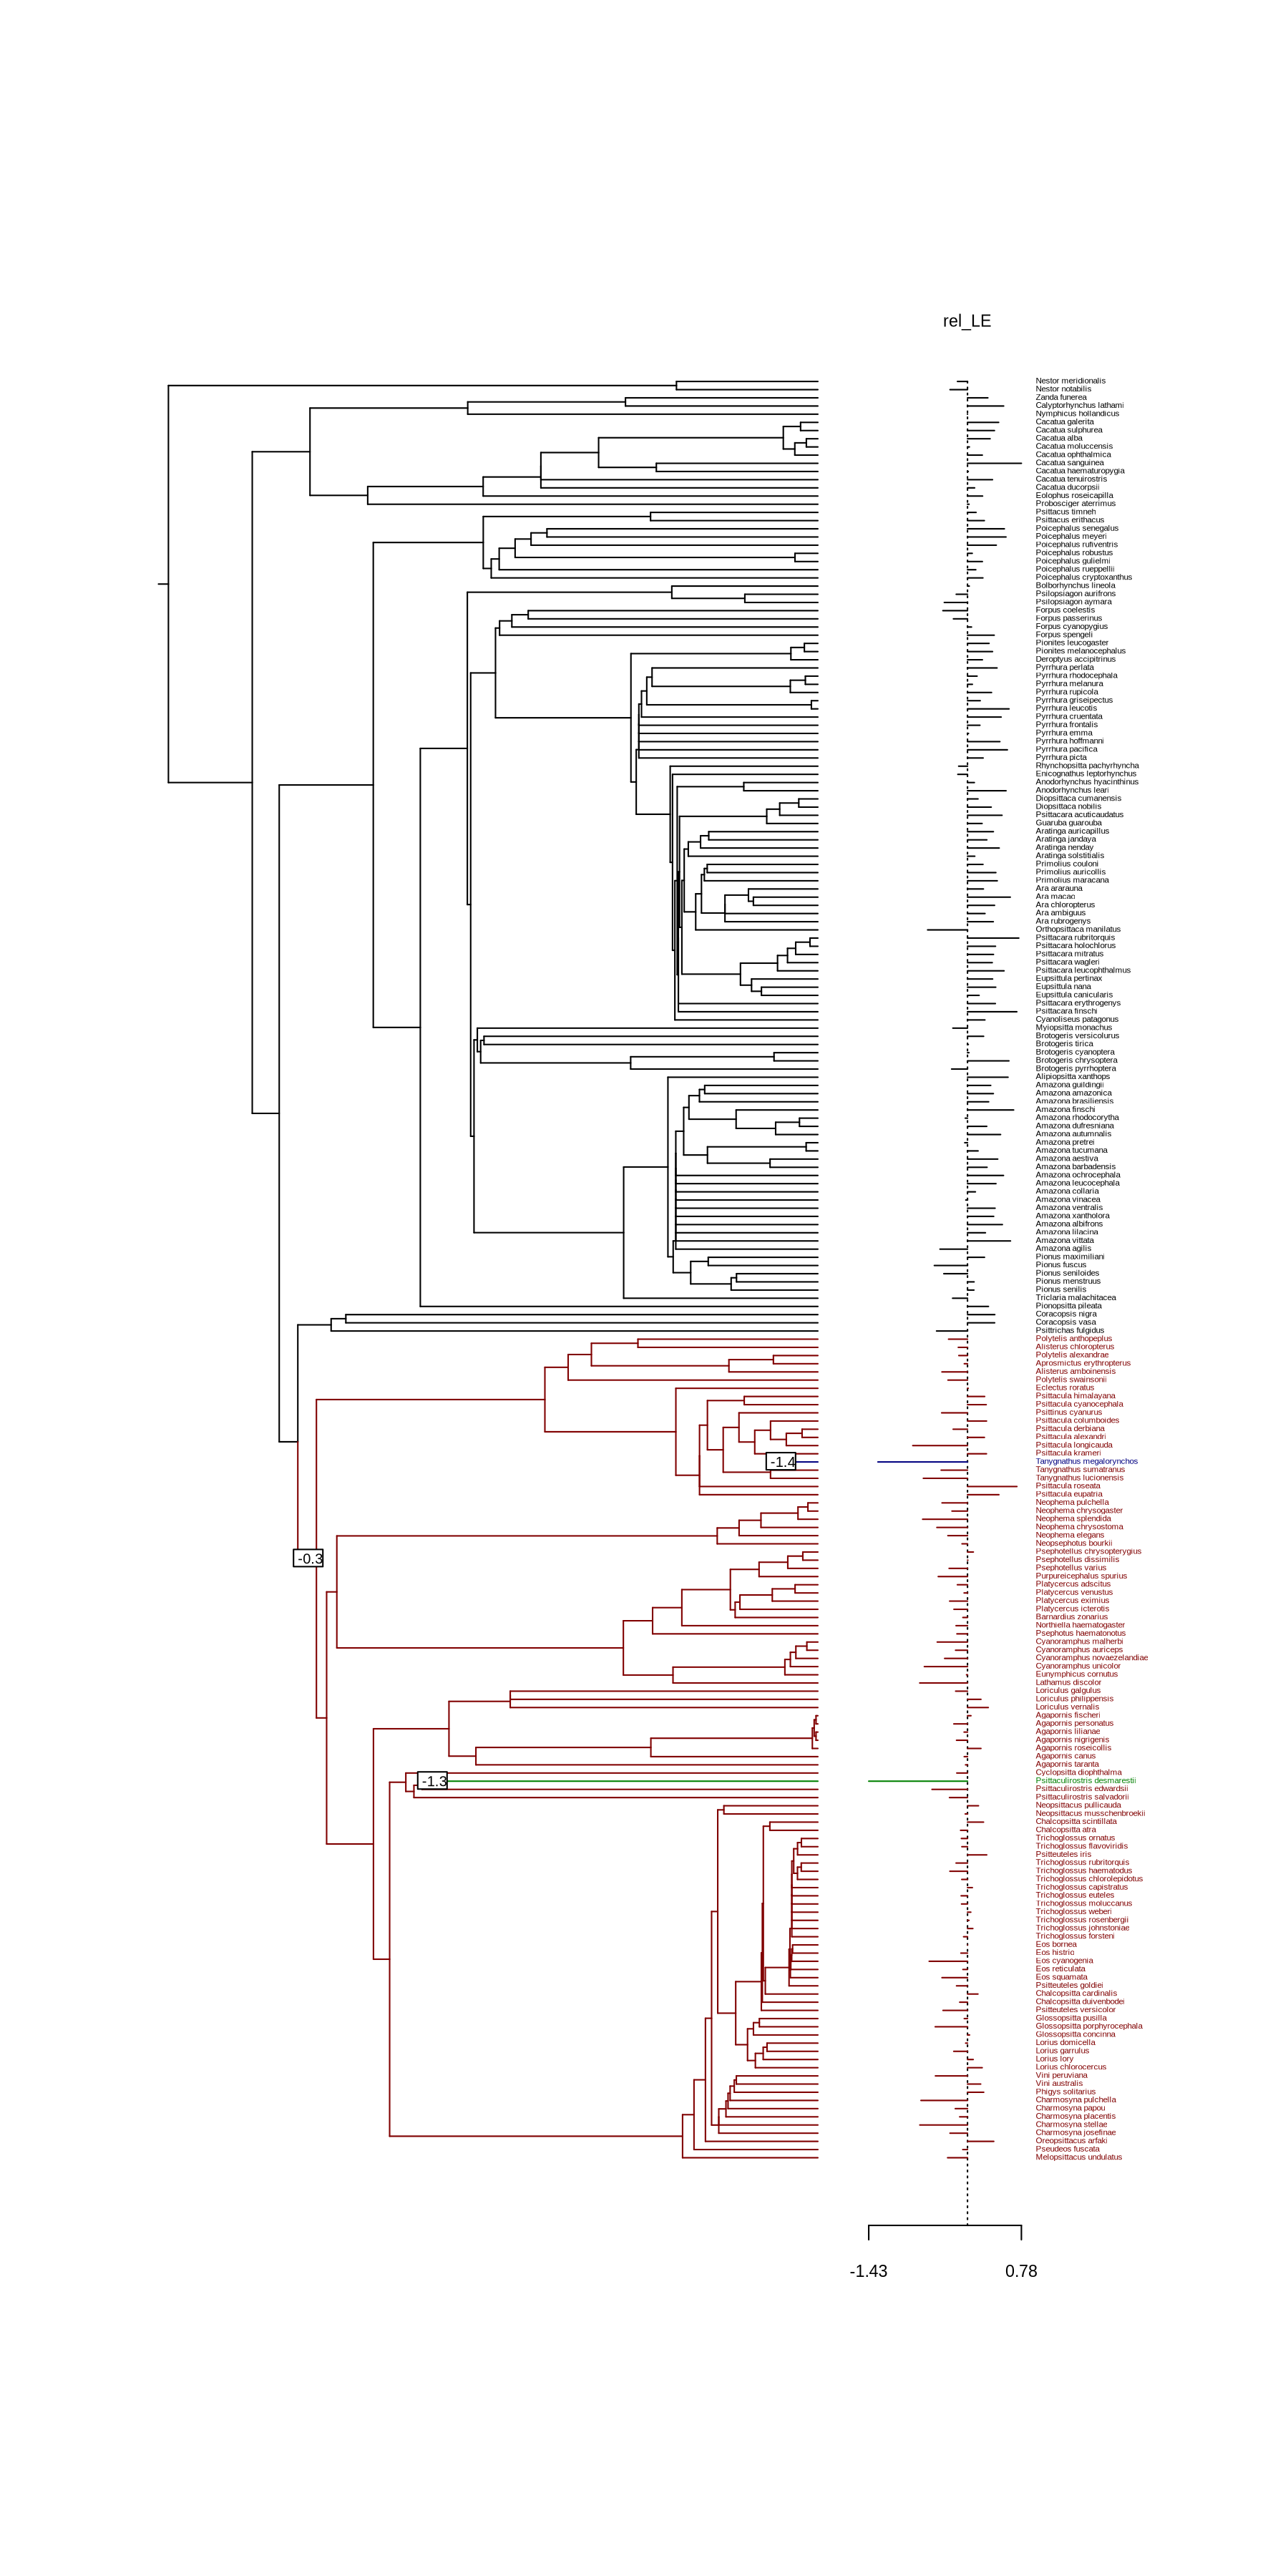
\includegraphics[width=0.48\textwidth]{../results/phase0b/figures/fig4_regime_shifts_rel_LE.png}
\caption{\textbf{Phase 0b Two-Outcome Sensitivity \& Regime Shifts:} (\textbf{Left}) Modest concordance ($\rho = 0.35$) between relative life expectancy and sample-size-adjusted maximum longevity across 138 parrots, showing outcome sensitivity in kea and macaws. (\textbf{Right}) \texttt{PhylogeneticEM} scOU inference ($K = 3$ reductions from ancestral optimum $+0.22$), led by a $-0.35$ log shift on the Psittaculidae stem ($p = 0.003$ Burgio vs.\ $p = 0.052$ Smith 2024).}
\label{fig:phase0b}
\end{figure*}

\section{Results}

\subsection{Macroevolution of Parrot Longevity and Necropsy Epidemiology (Phases 0 \& 0b)}
Across $218$ parrots, PGLS with Pagel's $\lambda = 0.65$ outperforms Brownian ($\Delta\text{AIC} = 69.9$) and single-optimum OU ($\Delta\text{AIC} = 14.9$) models, yielding an allometric slope of $0.349 \pm 0.032$ (\textbf{Fig.~\ref{fig:phase0}}, \textbf{Table~\ref{tab:phase0}}). Ancestral reconstruction under scOU (\texttt{PhylogeneticEM}, \textbf{Fig.~\ref{fig:phase0b}}, right) recovers an ancestrally long-lived regime (root optimum $+0.22$) sustained across Neotropical Arini (\textit{Psittacara}, \textit{Ara}, \textit{Anodorhynchus}), Androglossini (\textit{Amazona}), Cacatuidae, and Strigopidae, punctuated by three rate reductions led by the ancestral branch of Psittaculidae ($\Delta\theta = -0.35$, $n = 101$ descendant tips; direct PGLS indicator $-31\%, p = 0.003$). Crucially, switching to sample-size-corrected maximum longevity ($n = 152$, $\rho = 0.35$ against life expectancy; \textbf{Fig.~\ref{fig:phase0b}}, left) preserves only the Psittaculidae contrast ($-18\%, p = 0.03$, though $K = 0$ in scOU), and re-testing on the dated Smith et al.\ (2024) molecular tree elevates phylogenetic signal to $\lambda = 0.88$ while weakening the Psittaculidae longevity contrast to borderline significance ($\beta = -0.076 \pm 0.039$, $-25\%$, $p = 0.050$--$0.052$). Thus, clade-level longevity reduction in Psittaculidae represents a single topology-sensitive event.

Conversely, veterinary neoplasia epidemiology provides an unambiguous, topology-independent signal: \textit{Melopsittacus undulatus} is an extreme tumor outlier relative to all other parrots including fellow Psittaculidae lories (\textbf{Table~\ref{tab:phase0}}). In AZA records ($n = 5,729$ necropsies), budgerigars display $20.8\%$ neoplasia ($17.4\%$ malignant) versus $1.5\%$ ($0.8\%$ malignant) in lories (OR $= 17, p \approx 10^{-21}$; beta-binomial outlier $p = 0.002$). In the independent UC Davis database ($n = 10,152$ necropsies), age-standardized tumor prevalence in \textit{M.\ undulatus} reaches $25.9\%$ versus $5.4\%$ in lories ($4.8\times, p \approx 10^{-16}$) and $9.1\%$ in cockatiels (\textit{Nymphicus hollandicus}, $p \approx 10^{-17}$), ruling out domestication or captive age structure as sole explanations.

\begin{table}[h]
\centering
\caption{Phase 0/0b macroevolutionary allometry, topology sensitivity, and veterinary necropsy epidemiology.}
\label{tab:phase0}
\resizebox{\columnwidth}{!}{%
\begin{tabular}{llrr}
\toprule
\textbf{Analysis / Dataset} & \textbf{Model / Contrast} & \textbf{Estimate} & \textbf{$p$ / $\Delta$AIC} \\
\midrule
PGLS LE $\sim$ Mass ($n=218$) & Pagel's $\lambda = 0.65$ (slope) & $+0.349 \pm 0.032$ & $\Delta\text{AIC}=0$ \\
scOU Regime Shift (\texttt{Burgio}) & Ancestral Psittaculidae ($K=3$) & $-0.35$ (vs.\ $+0.22$) & LINselect \\
Psittaculidae LE Contrast & \texttt{Burgio 2019} / \texttt{Smith 2024} & $-31\%$ / $-25\%$ & $0.003$ / $0.050$ \\
Max Longevity Adj.\ ($n=152$) & Concordance with Rel.\ LE & Spearman $\rho = 0.35$ & $p = 0.03$ (Psl) \\
AZA Neoplasia ($n=5,729$) & \textit{M.\ undulatus} vs.\ Lories & 20.8\% vs.\ 1.5\% & OR=17, $10^{-21}$ \\
UC Davis Age-Std ($n=10,152$) & \textit{M.\ undulatus} vs.\ Lories / Cockatiel & 25.9\% vs.\ 5.4\% / 9.1\% & $10^{-16}$ / $10^{-17}$ \\
\bottomrule
\end{tabular}%
}
\end{table}

\subsection{Phase 1: Assembly Audit Uncovers Cross-Contamination and Yields 71 Species}
Completing \texttt{compleasm aves\_odb10}, mitogenome BLAST, and Mash nuclear audits across all $126$ assemblies (\textbf{Table~\ref{tab:audit}}; \textbf{Fig.~\ref{fig:audit}}; Table~S1) exposed pervasive batch quality failures in short-read drafts. Across $96$ Iridian assemblies, median completeness was $76.1\%$, and $0/31$ assemblies with $\text{contig N50} < 5\text{ kb}$ passed the $70\%$ cutoff. Critically, $61/96$ Iridian genomes contained complete foreign mitochondrial genomes ($88\%$ matching donors sequenced in the same Iridian batch, including reciprocal lab swaps), and four assemblies failed nuclear Mash identity: ``\textit{Agapornis nigrigenis}'' (\texttt{GCA\_035041115.1}) is a passerine (\textit{Garrulax}, nuclear Mash $\ge 0.145$), ``\textit{Aratinga jandaya}'' (\texttt{GCA\_026284485.1}) is \textit{Poicephalus meyeri} (Mash $= 0.0039$), and two assemblies (\textit{Cacatua haematuropygia}, \textit{Trichoglossus haematodus}) are chimeras contaminated with the same passerine DNA. Deduplicating and applying filters ($\text{BUSCO}_{\text{complete}} \ge 70\%$) finalized $71$ validated species ($58$ discovery + $13$ holdout; Table~S1), with zero technical correlation between assembly quality (`busco\_C` $p = 0.111$--$0.352$, `contig N50` $p = 0.198$--$0.249$, GC $p \ge 0.097$) and residual longevity.

\begin{figure}[t]
\centering
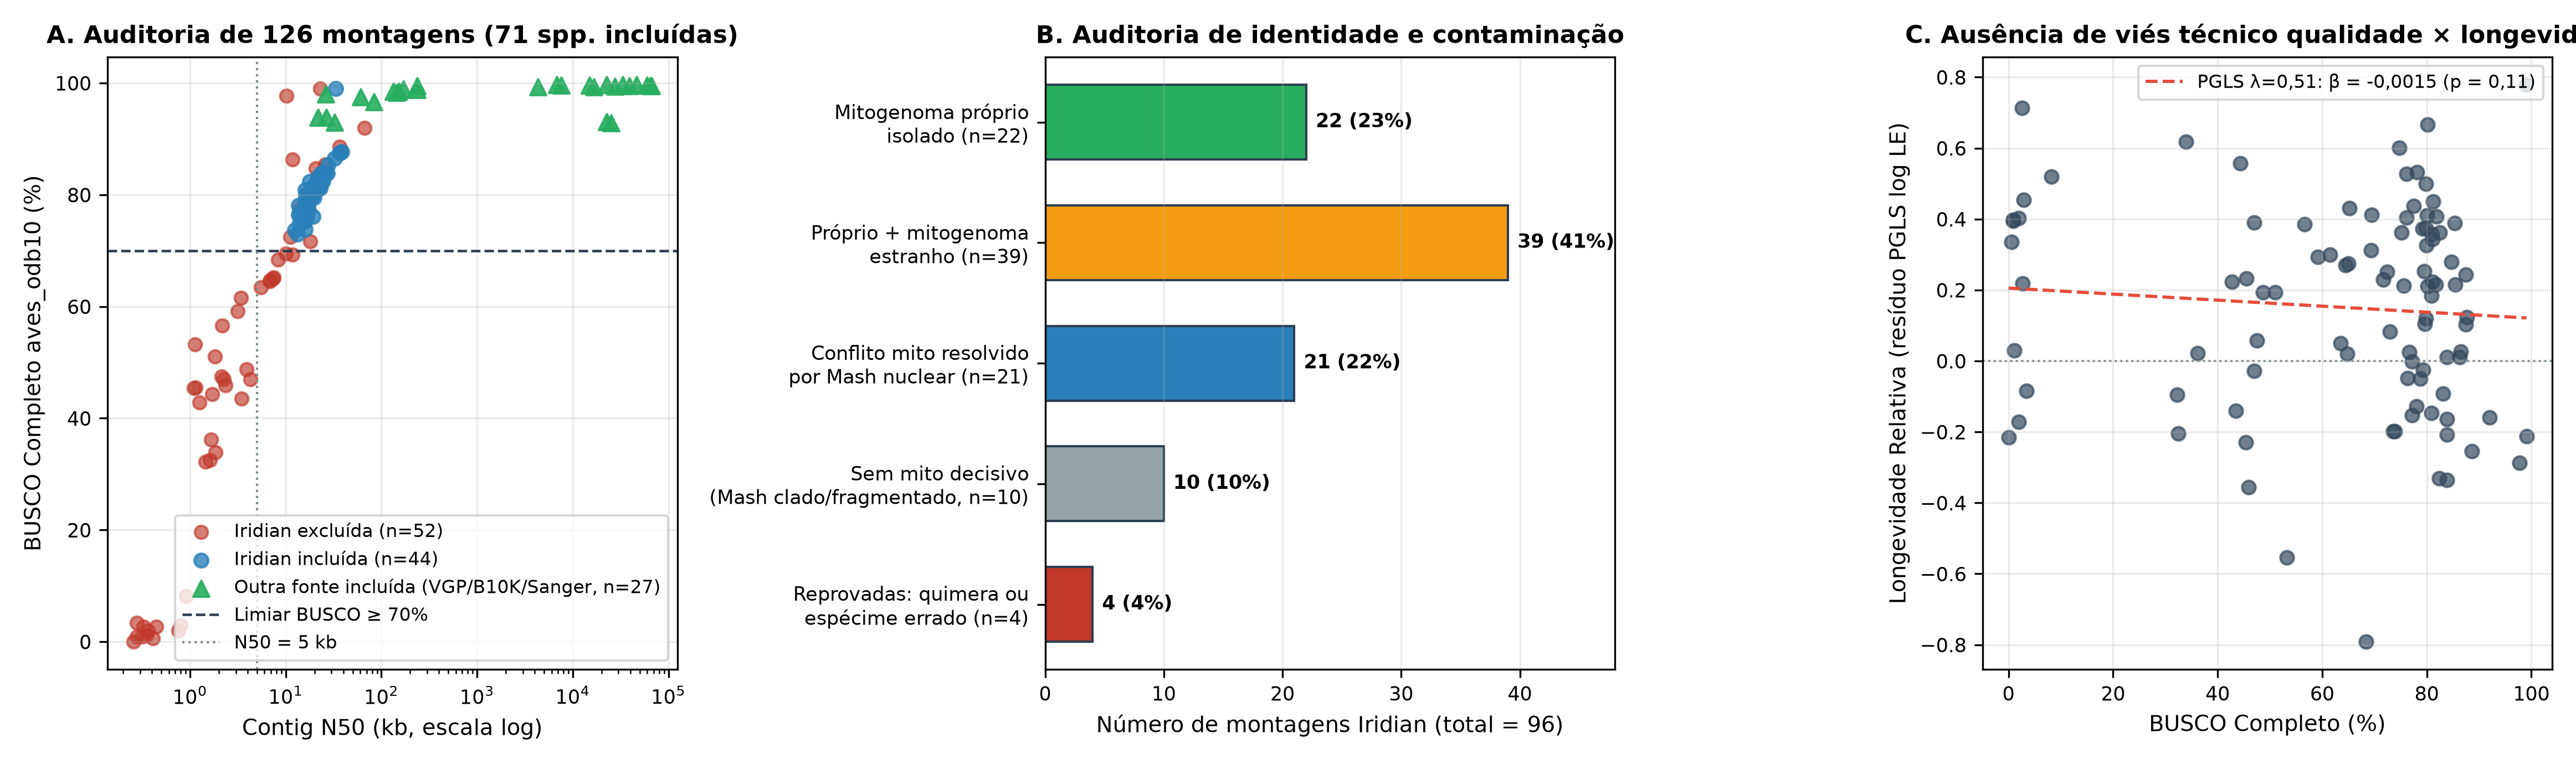
\includegraphics[width=\columnwidth]{../results/phase1_audit/figS1_audit_126_assemblies.png}
\caption{\textbf{Phase 1 Assembly Audit ($126$ assemblies / $105$ species):} \texttt{compleasm aves\_odb10} completeness against contig N50, highlighting exclusion of fragmented drafts ($<70\%$), nuclear swaps/chimeras, and absence of technical bias with relative longevity ($p \ge 0.11$).}
\label{fig:audit}
\end{figure}

\begin{table}[h]
\centering
\caption{Summary of the 126-assembly genomic audit (\texttt{species\_genomes.tsv}).}
\label{tab:audit}
\resizebox{\columnwidth}{!}{%
\begin{tabular}{lrr}
\toprule
\textbf{Audit Category / Quality Filter} & \textbf{Assemblies} & \textbf{Species} \\
\midrule
Total audited (\texttt{compleasm aves\_odb10}) & 126 & 105 \\
\quad Iridian short-read batch / Independent long-read & 96 / 30 & 96 / 29 \\
Excluded for $\text{BUSCO}_{\text{complete}} < 70\%$ & 39 & 32 \\
Excluded for nuclear swap / chimera (Mash) & 4 & 2 \\
\midrule
\textbf{Included species ($\text{BUSCO} \ge 70\%$)} & \textbf{71} & \textbf{71} \\
\quad Psittaculidae / Other Psittaciformes & 20 / 51 & 20 / 51 \\
\quad Strict original criterion ($\ge 85\%$ \& $\text{N50} \ge 20\text{ kb}$) & 33 & 33 \\
Frozen discovery panel (Phases 2--3) / Holdout set & 58 / 13 & 58 / 13 \\
\bottomrule
\end{tabular}%
}
\end{table}

\subsection{Phase 2: Refutation of Tumor-Suppressor Loss, Telomere Signal, 71-Species Confirmation, and Multi-Hit Collapse}
Across the $87$ alignable H8 panel genes in $58$ species ($97$ aligned across $71$ species; \textbf{Fig.~\ref{fig:phase2}}), we reject modular loss or relaxation of cancer-defense networks:
\begin{enumerate}
    \item \textbf{Zero confirmed pseudogenizations:} All $329$ apparent disruptions ($451$ in $71$ species; Table~S2) resolved as single-reference alignment artifacts (\texttt{OGG1}, \texttt{MUTYH}, \texttt{MYC}, \texttt{HMOX1}), heterozygous stop variants (\texttt{PSMD6} in \textit{Loriculus galgulus}: $21$ C vs.\ $20$ T SRA reads), or $0\times$ Illumina dropout across a $75$--$77\%$ GC exon 1 in \texttt{ACD} (\textit{Psittacus erithacus}). Because GC-rich \texttt{TP53} and \texttt{RB1} remained fragmented in short-read drafts (intact in only $4$ and $19$ of $71$ species), putative loss in those two genes remains untestable outside long-read assemblies.
    \item \textbf{Modular null benchmark:} Neither module heterogeneity in mean $\log_2 k$ ($p = 0.164$ Burgio, $0.955$ Smith) nor any module M1--M8 departed significantly from $1,000$ matched pseudo-panels sampled from $298$ genomic controls (lowest nominal M2 $p = 0.024$ was driven by two $k \approx 0$ boundary genes and collapsed to $p = 0.070$ under medians; Table~S3).
    \item \textbf{Telomeric (M7) episodic signal vs.\ Red-Team controls and 71-species confirmation:} Under standard \texttt{aBSREL}, $5/8$ ($62.5\%$) telomeric M7 genes (\texttt{RTEL1} $p = 1.73\times 10^{-10}$, \texttt{TERF2} $1.79\times 10^{-6}$, \texttt{TERT} $2.63\times 10^{-4}$, \texttt{ACD} $2.46\times 10^{-4}$, \texttt{TERF1} $3.98\times 10^{-4}$) and \texttt{MYC} ($1.69\times 10^{-8}$) reached $q < 0.10$ on \textit{M.\ undulatus} (BH-corrected across all $86$ tested panel genes), contrasting starkly with non-M7 panel modules ($1/78 = 1.3\%$) and $19$ control genes ($1/19 = 5.3\%$ nominal; \textbf{0/19 FDR}; Fisher $p = 0.00069$; $0/298$ controls had $\omega > 1$ in RELAX). In Psittaculidae, non-boundary RELAX intensification replicated in \texttt{TERT} ($k = 5.51/3.10$, $q = 0.0008/0.011$) and \texttt{MRE11} ($k = 2.60/2.61$, $q = 0.002/0.005$), with moderate relaxation in \texttt{DKC1} ($k = 0.49$) and \texttt{NQO1} ($k = 0.34$). Expanding alignments up to $71$ species (\textbf{Table~S2}; nearly doubling taxon sampling for \texttt{TERT} $15\to 34$, \texttt{RTEL1} $23\to 35$, \texttt{TERF2} $18\to 29$, \texttt{POT1} $8\to 26$, and \texttt{TERF1} $9\to 25$) sharpens the telomeric cluster while falsifying all non-telomeric RELAX hits except \texttt{NQO1}: \texttt{TERT} ($k = 2.24$, RELAX $p = 1.32\times 10^{-7}$; \texttt{aBSREL} $p = 1.04\times 10^{-4}$), \texttt{POT1} ($k$ strengthens from $1.94, p = 0.075$ to $8.17, p = 2.27\times 10^{-5}$), \texttt{DKC1} ($k = 0.55, p = 7.15\times 10^{-6}$), \texttt{RTEL1} (moves off the $k=0$ boundary to $k = 0.52, p = 0.0159$; \texttt{aBSREL} $p = 9.43\times 10^{-11}$), \texttt{TERF2} ($k = 0.59, p = 0.0161$; \texttt{aBSREL} $p = 5.95\times 10^{-5}$), and \texttt{NQO1} ($k = 0.71, p = 0.0091$) preserve their selective regimes, whereas \texttt{MRE11} ($49\to 63$ spp) collapses to non-significance ($k = 0.86, p = 0.106$), \texttt{SOD1} flips from apparent intensification ($k = 31.65$) to a zero boundary ($k = 3.8\times 10^{-6}$), and \texttt{CCNE1} reverses and becomes null ($k = 1.76, p = 0.229$).

    Crucially, however, Red-Team alignment auditing (\textbf{Table~\ref{tab:telomere_redteam}}) demonstrates that although \textit{S.\ habroptila} dual-reference coordinates verify $100\%$ single-locus orthology for \texttt{RTEL1} ($40/40$), \texttt{TERF2} ($30/30$), \texttt{TERT} ($35/35$), \texttt{TERF1} ($27/27$), and \texttt{POT1} ($27/27$) and \texttt{MAFFT L-INS-i} reproduces every signal, \textbf{cleaning gappy/noisy windows} ($>15\%$ gap columns and 10-codon windows with $\ge 3$ AA differences) extinguishes \texttt{RTEL1} ($p = 1.00$), \texttt{ACD} ($0.125$), and \texttt{TERF2} ($0.068$), leaving only \texttt{TERT} ($p = 0.0052$) and \texttt{TERF1} ($p = 0.0037$). Further allowing simultaneous multinucleotide changes (\texttt{-{}-multiple-hits Double+Triple}) collapses all five signals ($p = 0.967$--$1.00$; \texttt{ACD} $0.050$--$0.132$).
\end{enumerate}

\begin{figure*}[t]
\centering
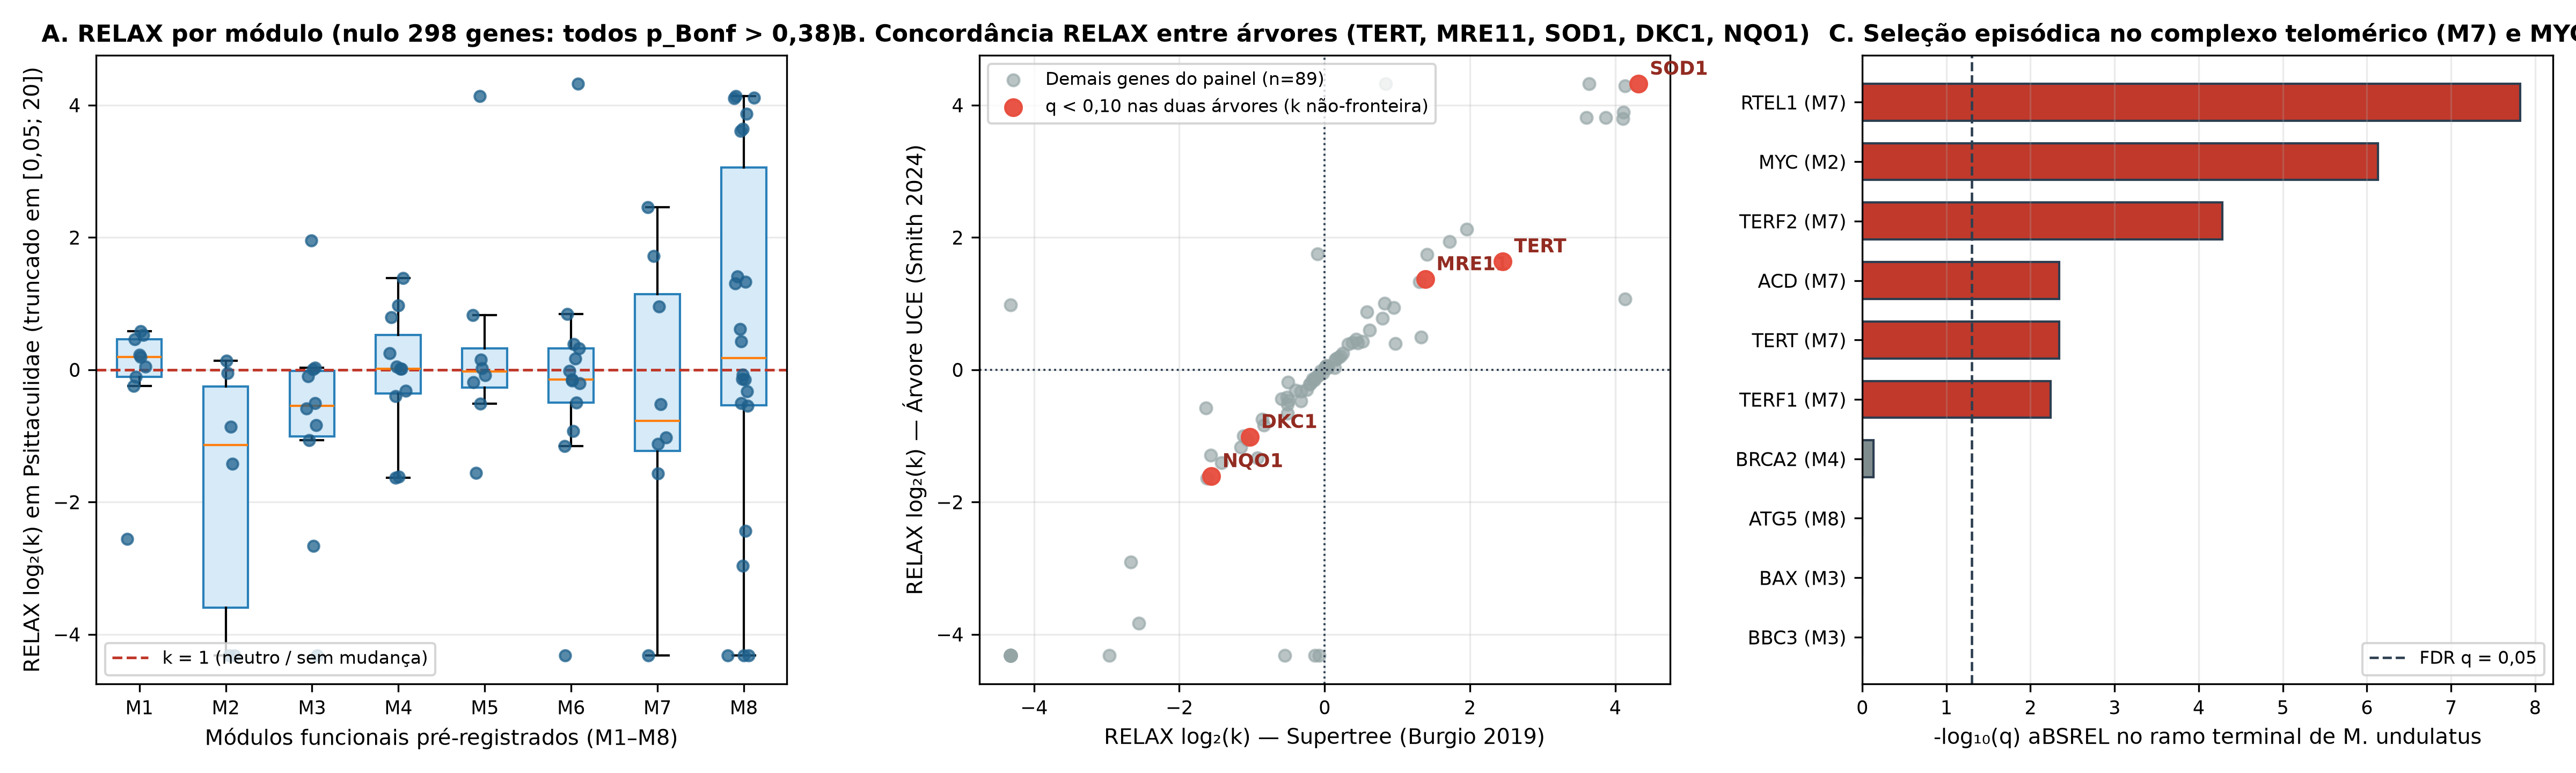
\includegraphics[width=0.90\textwidth]{../results/phase2_genes/fig5_phase2_selection_h8.png}
\caption{\textbf{Phase 2 Selection Tests (H8, 58 species):} (A) Module $\log_2 k$ distributions vs.\ 298-gene null model; (B) Per-gene RELAX significance; (C) Concentration of standard \texttt{aBSREL} calls in telomere genes (M7) and \texttt{MYC} prior to Red-Team window-cleaning and Multi-Hit auditing; (D) Resolution of apparent gene disruptions via second-reference and SRA read checks.}
\label{fig:phase2}
\end{figure*}

\begin{table*}[t]
\centering
\caption{Red-Team sensitivity audit of telomeric (M7) \texttt{aBSREL} signals on the \textit{M.\ undulatus} branch and dual-reference orthology verification (\texttt{7\_telomere\_alignment\_and\_rbh.tsv}).}
\label{tab:telomere_redteam}
\resizebox{\textwidth}{!}{%
\begin{tabular}{lccccccc}
\toprule
\textbf{Gene} & \textbf{Spp.} & \textbf{\textit{M.\ und.} AA Subs (Isolated / Noisy)} & \textbf{Orig.\ MAFFT $p$} & \textbf{L-INS-i $p$} & \textbf{Window-Cleaned $p$} & \textbf{Multi-Hit (\texttt{Double+Triple}) $p$} & \textbf{Kakapo Orthology} \\
\midrule
\texttt{RTEL1} & 23 & 279 (58 / 221) & $1.73\times 10^{-10}$ & $1.28\times 10^{-9}$ & \textbf{1.0000} & \textbf{0.9670} & 40/40 (2 loci \textit{Melo}) \\
\texttt{TERF2} & 18 & 89 (32 / 57) & $1.79\times 10^{-6}$ & $2.44\times 10^{-6}$ & \textbf{0.0677} & \textbf{1.0000} & 30/30 \\
\texttt{TERT}  & 15 & 196 (95 / 101) & $2.63\times 10^{-4}$ & $1.12\times 10^{-4}$ & \textbf{0.0052} & \textbf{1.0000} & 35/35 \\
\texttt{ACD}   & 6  & 102 (42 / 60) & $2.46\times 10^{-4}$ & $1.23\times 10^{-4}$ & \textbf{0.1248} & \textbf{0.0502} (0.1320 cl.) & 8/11 (2 loci \textit{Melo}) \\
\texttt{TERF1} & 9  & 23 (15 / 8) & $3.98\times 10^{-4}$ & $1.99\times 10^{-4}$ & \textbf{0.0037} & \textbf{1.0000} (0.3151 cl.) & 27/27 \\
\texttt{POT1}  & 8  & 84 (52 / 32) & 1.0000 & 1.0000 & 1.0000 & 1.0000 & 27/27 \\
\bottomrule
\end{tabular}%
}
\end{table*}

\begin{figure*}[t]
\centering
\includegraphics[width=0.92\textwidth]{../results/phase3_genome/fig7_structural_3d_mapping.png}
\caption{\textbf{AlphaFold 3D Structural \& PAE Domain Mapping (Step 2):} Budgerigar substitutions distribute across ssDNA-binding OB1--OB3/HJRL domains in \texttt{POT1} ($58$ sites, mean pLDDT $= 72.6$) and cluster heavily in the C-terminal Harmonin-N/PIP region of \texttt{RTEL1} ($115/158$ sites), whereas \texttt{PTEN} exhibits 100\% invariance across its catalytic P-loop (\texttt{H123--R130}, pLDDT $= 93.0$) and Phosphatase+C2 core (residues 14--350).}
\label{fig:3d_mapping}
\end{figure*}

\subsection{AlphaFold 3D Structural Mapping}
Projecting alignment substitutions onto PAE-partitioned AlphaFold models (\textbf{Fig.~\ref{fig:3d_mapping}}; Table~S6) separates C-terminal/surface remodeling from ultra-conserved enzymatic pockets. In \texttt{RTEL1} ($1,219$ AA, global pLDDT $= 71.67$), $43$ budgerigar-specific changes fall within the N-terminal Rad3/FeS/Arch helicase core (residues $1$--$758$) whereas $115$ concentrate in the C-terminal Harmonin-N and PIP/RING region ($893$--$1,219$). In \texttt{POT1} ($780$ AA, global pLDDT $= 79.21$), $34$ substitutions map across OB1/OB2 and $16$ across TPP1-binding OB3/HJRL (mean mutated-site pLDDT $= 72.6$). By contrast, \texttt{PTEN} ($403$ AA, pLDDT $= 82.47$) is 100\% invariant across its catalytic P-loop (\texttt{H123--R130}, pLDDT $= 93.0$) and Phosphatase+C2 superdomain ($14$--$350$), with polymorphisms restricted to its disordered C-tail ($351$--$403$, pLDDT $= 35.1$), matching \texttt{MAD2L2}'s rigidly conserved HORMA core (pLDDT $= 90.39$).

\begin{figure*}[t]
\centering
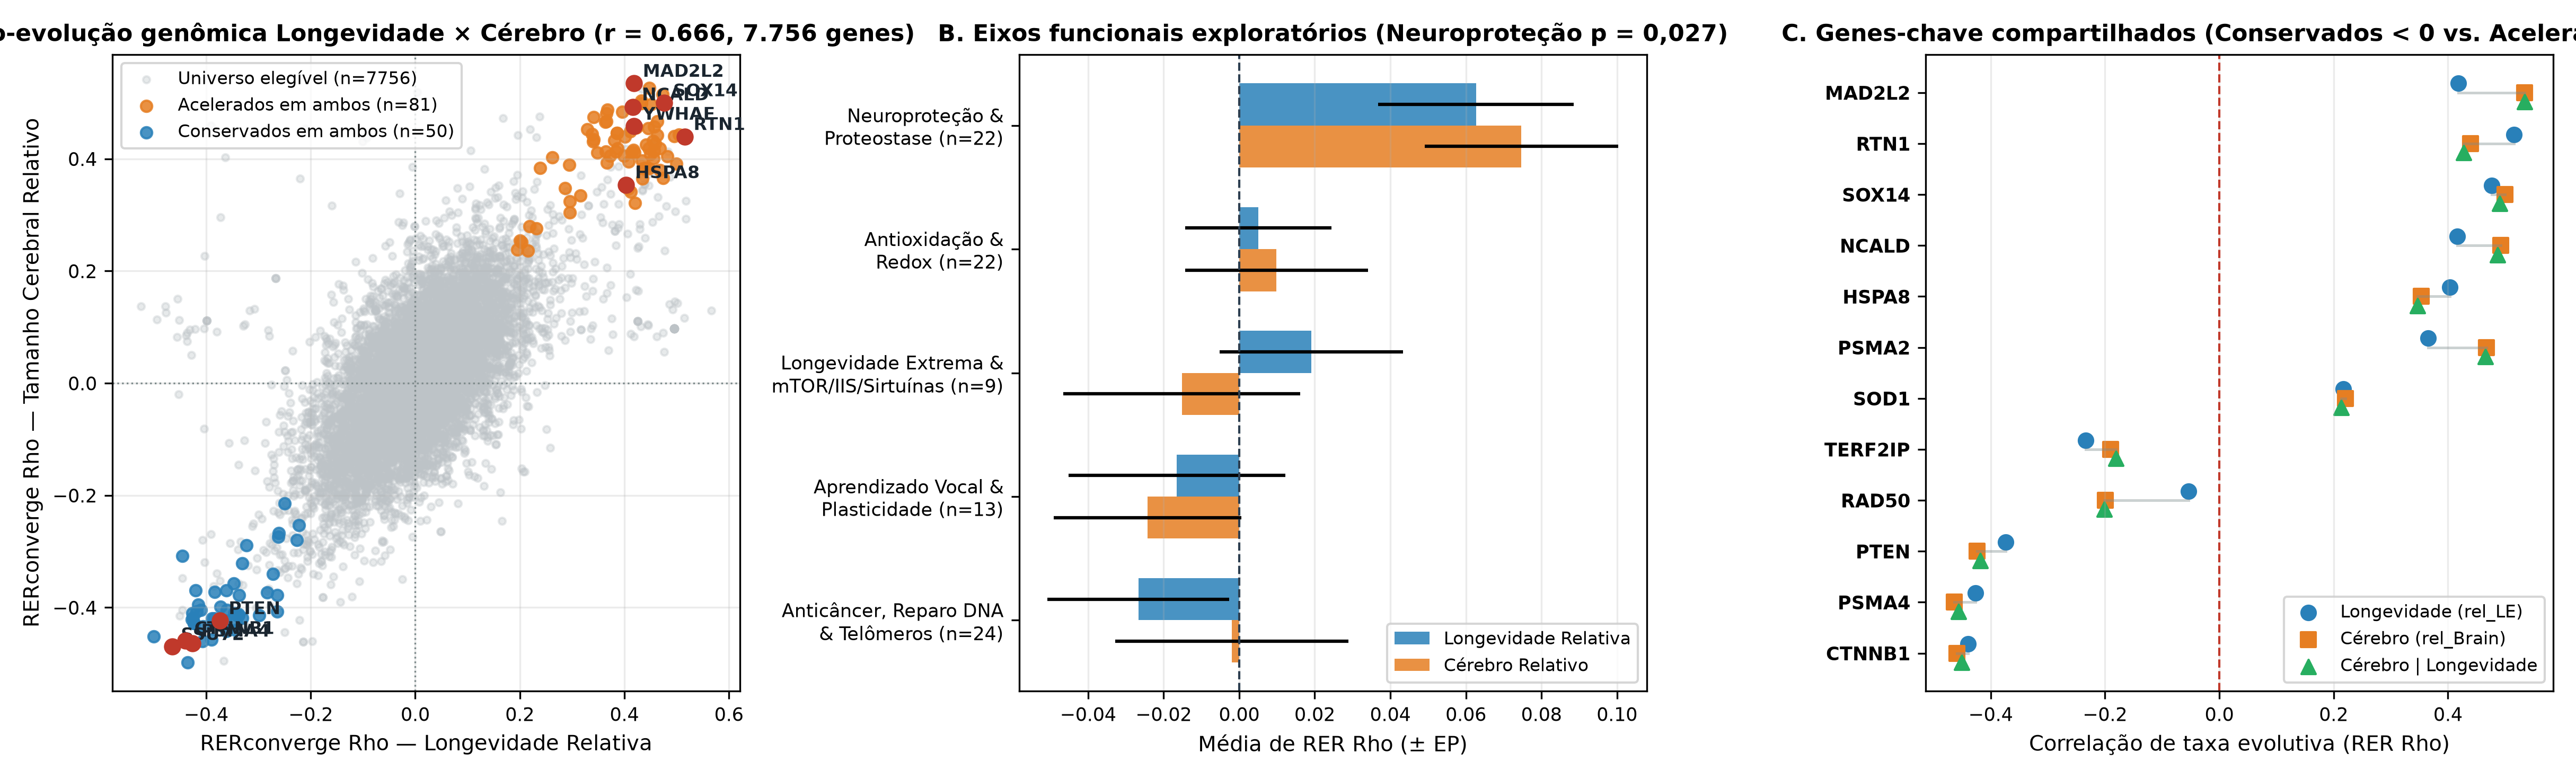
\includegraphics[width=0.94\textwidth]{../results/phase3_genome/fig6_phase3_genome_rer.png}
\caption{\textbf{Phase 3 Genome-Wide \texttt{RERconverge} Across $7,756$ Genes:} (A) Unadjusted genome-wide correlation ($r = 0.666$) between $\text{Rho}_{\text{LE}}$ and $\text{Rho}_{\text{Brain}}$; (B) Shared candidate rankings; (C) Exploratory functional axis shifts highlighting Neuroprotection/Proteostasis ($p = 0.014$--$0.046$); (D) Within-clade H8 results.}
\label{fig:phase3}
\end{figure*}

\subsection{Phase 3 (\texttt{RERconverge}): Genome Coupling, Orthogonalization, and Zero-Branch Artifacts}
Across $7,756$ genes in $58$ species (\textbf{Fig.~\ref{fig:phase3}}), $190$--$277$ genes per trait passed parametric $q < 0.10$, yet zero reached genome-wide permulation FDR ($\text{permQ} < 0.10$) owing to phylogenetic conservatism and the $1,000$-permulation resolution floor ($\text{permP}_{\min} = 0.001996$). Among $1,780$ GO terms, nominal directional consistency across both trees emerged in DNA recombination ($p = 3.2\times 10^{-4}$), DNA damage response ($p = 0.0076$), telomere maintenance ($p = 0.013$), mitochondrial translation ($p = 0.0021$), macroautophagy ($p = 0.030$), and synaptic vesicle recycling ($p = 0.0030$), and among six exploratory functional axes only Neuroprotection \& Proteostasis shifted above background in both traits ($p = 0.014$--$0.046$).

Unadjusted trait-RER correlations across all $7,756$ genes correlate strongly ($r = 0.666$ Burgio, $0.667$ Smith, $0.748$ on the matched $50$-species matrix), are 100\% deterministic ($\max|\Delta\text{Rho}| = 5\times 10^{-16}$ across seeds), and persist after removing $14$ linear, log, and quadratic technical confounders ($r = 0.653$; $0.630$--$0.696$ across quartiles). Nevertheless, our Red-Team audit (\textbf{Table~\ref{tab:rer_redteam}}; Tables~S4--S5) exposes three essential caveats:
\begin{enumerate}
    \item \textbf{True partial orthogonalization halves the residual brain signal:} Subtracting an unwhitened PGLS slope ($\hat{\beta}_{\text{GLS}} = 0.040, \lambda = 0.90$) left \texttt{rel\_brain\_given\_le} correlated with longevity at $r_{\text{tip}} = 0.427$ ($\text{cor}(\text{Rho}_{\text{Brain}}, \text{Rho}_{\text{PGLS}}) = 0.999$), explaining why $r$ fell only from $0.666$ to $0.639$. Applying true tip-OLS orthogonalization ($\hat{\beta}_{\text{OLS}} = 0.258, r_{\text{tip}} = 0$) cuts $r$ in half to \textbf{0.332} ($0.369$ in 50sp), and branch-path orthogonalization ($r_{\text{path}} = 0$) gives \textbf{0.389}. Furthermore, Brownian permulations yield a wide null SD ($0.29$--$0.35$, max $+0.716$, empirical $p = 0.010$--$0.025$) because genome-wide branch-rate covariance amplifies any shared branch-path correlation into $r_{\text{Rho}}$ ($\text{cor}(r_{\text{Rho}}, r_{\text{path}}) = 0.883$--$0.913$), whereas mass-orthogonalized clutch size drops to the noise floor ($r = -0.102$).
    \item \textbf{Clade dependence:} Dropping any single clade leaves $r_{\text{Rho}} \in [0.649, 0.798]$, but removing all $13$ Psittaculidae drops phenotypic $r_{\text{tip}}$ from $0.478$ to \textbf{0.195} (Spearman \textbf{0.097}) and $r_{\text{Rho}}$ from $0.748$ to \textbf{0.522}.
    \item \textbf{Zero-branch invariance drives 89.3\% of shared single-gene hits:} Total tree length negatively correlates with signed $\text{Rho}_{\text{Brain}}$ ($r = -0.178, p = 1.8\times 10^{-56}$). Crucially, \textbf{117/131 (89.3\%)} shared significant hits (\textbf{Tier~A}: \texttt{PTEN}, \texttt{MAD2L2}, \texttt{HSPA8}, \texttt{CTNNB1}, \texttt{SOX14}, \texttt{RTN1}, \texttt{PSMA4}) possess \textbf{97--99\% zero-length branches ($\le 10^{-6}$)}. Their studentized residuals mirror $\pm\sqrt{\text{nv}}$ from the genome background average—accounting for why \texttt{PTEN} flips from $-0.374$ to $+0.184$ when normalized within a small 91-gene panel yet holds 100\% sign concordance across 30 within-cohort CV splits sharing \texttt{nv}. Restricting to \textbf{Tier~B informative genes} ($\ge 20$ nonzero branches, $n = 6,182$) retains $14$ shared hits (\textbf{Table~\ref{tab:tierb}}; Table~S5), led by \texttt{TKT}, \texttt{PHOSPHO1}, \texttt{TADA2A}, \texttt{SLC4A7}, and \texttt{HUS1}.
\end{enumerate}

\begin{table}[h]
\centering
\caption{Red-Team stress tests on Phase 3 genome-wide coupling $r(\text{Rho}_{\text{LE}}, \text{Rho}_{\text{Brain}})$.}
\label{tab:rer_redteam}
\resizebox{\columnwidth}{!}{%
\begin{tabular}{lccc}
\toprule
\textbf{Audit Test / Perturbation} & \textbf{$r_{\text{tip}}$} & \textbf{$r_{\text{path}}$} & \textbf{$r(\text{Rho}_1, \text{Rho}_2)$} \\
\midrule
Original (\texttt{seed=20261028}) / \texttt{seed=999999} & +0.478 & +0.415 & \textbf{0.6663 / 0.6663} \\
50-species matched \texttt{rers\_50} matrix & +0.478 & +0.425 & \textbf{0.7478} \\
Adjusted for 14 quadratic+log confounders & -- & -- & \textbf{0.6532} \\
\midrule
Negative control: mass-resid.\ clutch size ($n=51$) & -0.173 & -0.214 & \textbf{-0.1024} \\
200 BM permulations (independent pairs) & $\sim 0$ & -0.002 & SD=0.289, $p=0.010$ \\
Observed LE $\times$ 200 Brain permulations & $\sim 0$ & +0.033 & SD=0.350, $p=0.025$ \\
\midrule
Leave-one-clade-out: Drop \textit{M.\ undulatus} (-1) & +0.446 & +0.405 & 0.7285 \\
Leave-one-clade-out: Drop Arini (-12) & +0.380 & +0.241 & 0.6489 \\
Leave-one-clade-out: \textbf{Drop Psittaculidae (-13)} & \textbf{+0.195} & \textbf{+0.209} & \textbf{0.5225} \\
\midrule
Unwhitened PGLS \texttt{rel\_brain\_given\_le} & +0.427 & +0.370 & 0.6385 \\
\textbf{True Tip-OLS orthogonalization ($r_{\text{tip}}=0$)} & \textbf{0.000} & -0.063 & \textbf{0.3322} \\
\textbf{True Branch-path orthogonalization ($r_{\text{path}}=0$)} & -- & \textbf{0.000} & \textbf{0.3888} \\
Analytical per-gene partial correlation & -- & 0.000 & \textbf{0.4135} \\
\bottomrule
\end{tabular}%
}
\end{table}

\begin{table}[h]
\centering
\caption{Selected Tier~A (ultra-conserved $>97\%$ zero branches) vs.\ top Tier~B ($\ge 20$ nonzero branches) shared candidates ($P < 0.05$ \& $\text{permP} < 0.05$ for both longevity and brain; full list in Table~S5).}
\label{tab:tierb}
\resizebox{\columnwidth}{!}{%
\begin{tabular}{llcccc}
\toprule
\textbf{Gene} & \textbf{Tier (\% Zero Br.)} & \textbf{$\text{Rho}_{\text{LE}}$} & \textbf{$\text{permP}_{\text{LE}}$} & \textbf{$\text{Rho}_{\text{Brain}}$} & \textbf{$\text{permP}_{\text{Brain}}$} \\
\midrule
\texttt{PTEN}   & Tier A (99.1\%, 1 nz) & -0.374 & 0.0080 & -0.424 & 0.010 \\
\texttt{MAD2L2} & Tier A (99.0\%, 1 nz) & +0.418 & 0.0120 & +0.534 & 0.002 \\
\texttt{HSPA8}  & Tier A (98.2\%, 2 nz) & +0.404 & 0.0080 & +0.354 & 0.030 \\
\texttt{CTNNB1} & Tier A (99.1\%, 1 nz) & -0.439 & 0.0040 & -0.459 & 0.012 \\
\midrule
\texttt{TKT}      & Tier B (60.9\%, 27 nz) & +0.408 & 0.0040 & +0.347 & 0.032 \\
\texttt{PHOSPHO1} & Tier B (52.3\%, 53 nz) & -0.261 & 0.0120 & -0.267 & 0.024 \\
\texttt{TADA2A}   & Tier B (72.6\%, 20 nz) & +0.316 & 0.0220 & +0.334 & 0.012 \\
\texttt{SLC4A7}   & Tier B (44.8\%, 37 nz) & +0.296 & 0.0319 & +0.304 & 0.046 \\
\texttt{HUS1}     & Tier B (54.1\%, 51 nz) & -0.222 & 0.0120 & -0.253 & 0.018 \\
\texttt{DEPDC4}   & Tier B (21.5\%, 73 nz) & -0.250 & 0.0100 & -0.214 & 0.034 \\
\bottomrule
\end{tabular}%
}
\end{table}

\section{Discussion}

Our integrated audit reconciles biological signal with methodological artifacts across three levels of avian comparative genomics:
\begin{enumerate}
    \item \textbf{Genome auditing is non-negotiable for public short-read drafts:} The prevalence of foreign mitochondrial genomes ($61/96$) and passerine contamination/chimerism ($3/96$) in batch-deposited genomes demonstrates that reliance on NCBI metadata without nuclear Mash and multi-reference exon validation will generate spurious claims of gene loss and episodic selection.
    \item \textbf{Budgerigar telomere divergence involves clustered/multinucleotide dynamics rather than gene loss:} Short-lived parrots retain intact DNA-repair and checkpoint toolkits. While M7 telomeric genes (\texttt{TERT}, \texttt{TERF1}, \texttt{RTEL1}, \texttt{TERF2}, \texttt{ACD}) show true orthology with \textit{Strigops} and exceed empirical control rates under standard \texttt{aBSREL}, sensitivity to noisy-window masking and complete absorption under \texttt{Double+Triple} multi-hit models suggest clustered multinucleotide mutational regimes or alignment-local divergence in C-terminal \texttt{RTEL1} and OB-domain \texttt{POT1} rather than classic dispersed positive selection. Targeted long-read sequencing and functional telomere-length assays in Psittaculidae remain key priorities, alongside resolving GC-rich \texttt{TP53} and \texttt{RB1} in chromosome-scale genomes.
    \item \textbf{Conserved proteomes challenge branch-rate correlation interpretation:} Even after proper OLS/branch-path orthogonalization ($r = 0.33$--$0.39$), brain size and lifespan remain partially coupled through shared rate structure on the parrot tree—anchored heavily by Psittaculidae versus long-lived radiations. Critically, future \texttt{RERconverge} applications on deeply conserved vertebrate proteomes must filter invariant genes ($>80\%$ zero-length branches), where studentized residuals mirror $-\hat{b}_g\sqrt{\text{nv}}$ rather than gene-specific convergent substitutions.
\end{enumerate}

\section*{Data \& Dashboard Availability}
Full scripts, confirmatory 71-species outputs, Supplementary Materials (\texttt{supplementary\_parrots\_EN.pdf}, Tables~S1--S6), Red-Team audit logs, and an interactive offline HTML raw-data explorer (\texttt{parrots\_raw\_data\_dashboard.html}) are hosted at \texttt{github.com/redkk123/Parrots} (branch \texttt{claude/new-session-lwh7xh}).

\begin{thebibliography}{9}
\footnotesize
\bibitem{burgio2019} Burgio, K.\ R.\ et al.\ (2019). Phylogenetic supertree and functional trait database for all extant parrots. \textit{Data in Brief}, 24, 103882.
\bibitem{kapsetaki2024} Kapsetaki, S.\ E.\ et al.\ (2024). Life history and cancer prevalence across vertebrates and avian clades. \textit{Cancer Discovery / Comparative Oncology}.
\bibitem{kowalczyk2019} Kowalczyk, A.\ et al.\ (2019). RERconverge: an R package for associating evolutionary rates with convergent traits. \textit{Bioinformatics}, 35(22), 4815--4817.
\bibitem{smith2024} Smith, B.\ T.\ et al.\ (2024). Phylogenomic calibration and macroevolutionary dynamics of Psittaciformes. \textit{Systematic Biology}.
\bibitem{wertheim2015} Wertheim, J.\ O.\ et al.\ (2015). RELAX: detecting relaxed selection in a phylogenetic framework. \textit{Molecular Biology and Evolution}, 32(3), 820--832.
\bibitem{wirthlin2018} Wirthlin, M.\ et al.\ (2018). Parrot genomes and the evolution of heightened longevity and cognition. \textit{Current Biology}, 28(24), 4001--4008.
\end{thebibliography}

\end{document}
